\title{Midterm for Electromagnetic Theory (PHYS330)}
\author{Dr. Jordan Hanson - Whittier College Dept. of Physics and Astronomy}
\date{\today}
\documentclass[10pt]{article}
\usepackage[a4paper, total={18cm, 27cm}]{geometry}
\usepackage{amsmath}
\usepackage{graphicx}
\usepackage{hyperref}
\begin{document}
\maketitle

\begin{abstract}
This exam may be completed at home, and covers chapters 1-3 of the course text and in-class examples.  Class notes and the course text may be used (open book), but no internet sources are allowed.  The daily warm-up exercises are good study materials for this exam.
\end{abstract}
\noindent

\section{Math Bootcamp}

\begin{enumerate}
\item (a) If $\mathbf{A}$ and $\mathbf{B}$ are two vector functions, what does the expression $(\mathbf{A} \cdot \nabla) \mathbf{B}$ mean?  That is, what are its $x$, $y$, and $z$ components, in terms of the Cartesian components of $\mathbf{A}$, $\nabla$, and $\mathbf{B}$? (b) Compute $(\hat{r} \cdot \nabla) \hat{r}$, where $\hat{r}$ is $\mathbf{r}/r$. (c) One can show that the \textit{force} on a dipole induced by a non-uniform field is
\begin{equation}
\mathbf{F} = (\mathbf{p} \cdot \nabla) \mathbf{E}
\end{equation}
Compute the force on a physical dipole located at the origin with $\mathbf{p} = q \mathbf{d} = qd~\mathbf{\hat{x}}$ in a field with associated potential $V(\mathbf{r}) = V_0 r^2 + V_1$. \\ \vspace{5cm}
\item Evaluate the following integral using (a) the three-dimensional Dirac delta function, or (b) integration by parts.  Solving both earns a bonus point.
\begin{equation}
J = \int_{\mathcal{V}} e^{-r} \left( \nabla \cdot \frac{\mathbf{\hat{r}}}{r^2} \right)
\end{equation} \\ \vspace{5cm}
\end{enumerate}

\clearpage

\section{Electrostatics}

\begin{enumerate}
\item Suppose two dipoles, each with dipole moment $\mathbf{p}$ pointed in opposite directions, form a square with alternating positive and negative charges and side length $d$.  Calculate the field $\mathbf{E}_{\rm tot}$ at the following points $P$: (a) $P = (0,0)$, (b) $P = (2d,0)$, and $P = (0,2d)$.  Check units and take limits\footnote{This object is an electrostatic quadrupole.}.  \\ \vspace{5cm}
\item The electric potential of some configuration is given by the expression
\begin{equation}
V(\mathbf{r}) = A \frac{e^{-\lambda r}}{r} \label{eq:lambda}
\end{equation}
In Eq. \ref{eq:lambda}, $A$ and $\lambda$ are constants.  Find the field $\mathbf{E}(\mathbf{r})$, the charge density $\rho$ and the total charge $Q$ in terms of $A$ and $\lambda$.  \textit{Hint: $\rho = \epsilon_0 A(4\pi\delta^3(\mathbf{r}) - \lambda^2\exp(-\lambda r)/r)$.} \textbf{Bonus:} compute the total energy stored in the field over all space. \\ \vspace{5cm}
\item (a) Use Gauss' Law to compute the field $\mathbf{E}$ as a function of the distance $s$ from a long straight wire with positive charge density $\lambda$. (b) Calculate the position versus time of a positive point charge $q$ with mass $m$ if it is released a distance $s$ from the wire. \\ \vspace{5cm}
\end{enumerate}

\clearpage

\section{Potentials}

\begin{enumerate}
\item Suppose the potential $V_0(\theta)$ at the surface of a sphere of radius $R$ is specified, and there is no charge inside or outside the sphere.  (a) Show that the charge density on the sphere is given by
\begin{align}
\sigma(\theta) &= \frac{\epsilon_0}{2R} \sum_{l=0}^{\infty} (2l+1)^2 C_l P_l(\cos\theta) \\
C_l &= \int_0^{\pi} V_0(\theta) P_l (\cos\theta) \sin\theta d\theta
\end{align}
(b) Produce the specific result for $\sigma(\theta)$ with $V_0(\theta) = P_2(\cos\theta)$. \\ \vspace{4cm}
\item For the infinite rectangular pipe in Example 3.4 from the text, suppose the constant potential $V_0$ is now only on one side.  That is, at $y=0$ and $x=\pm b$, the potential is zero.  At $y=a$, the potential is $V_0$.  Find the potential $V(x,y)$ inside the pipe.  \textit{Square pipes are examples of electromagnetic waveguides often used in microwave electronics.} \\ \vspace{4cm}
\item Consider Fig. \ref{fig:dipoles}.  Using the monopole and dipole potentials in the multipole expansion, find the approximate potential in spherical coordinates for each charge arrangement, far from the origin.  \textit{Note: these arrangements may or may not have a monopole moment in addition to the dipole moment.}
\begin{figure}
\centering
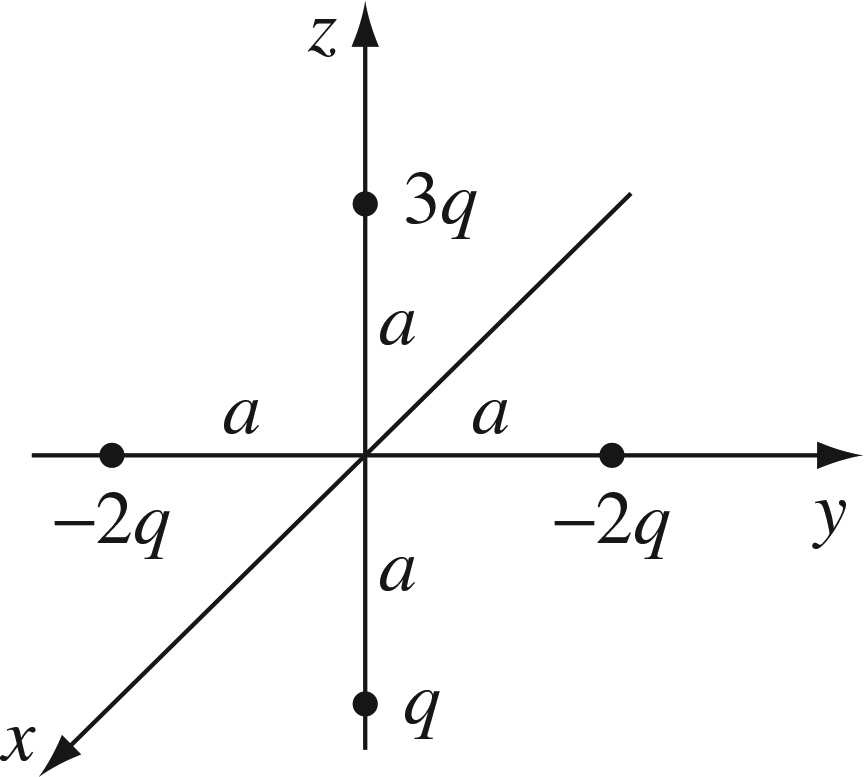
\includegraphics[width=0.225\textwidth]{figures/3_31.jpg} \hspace{1cm}
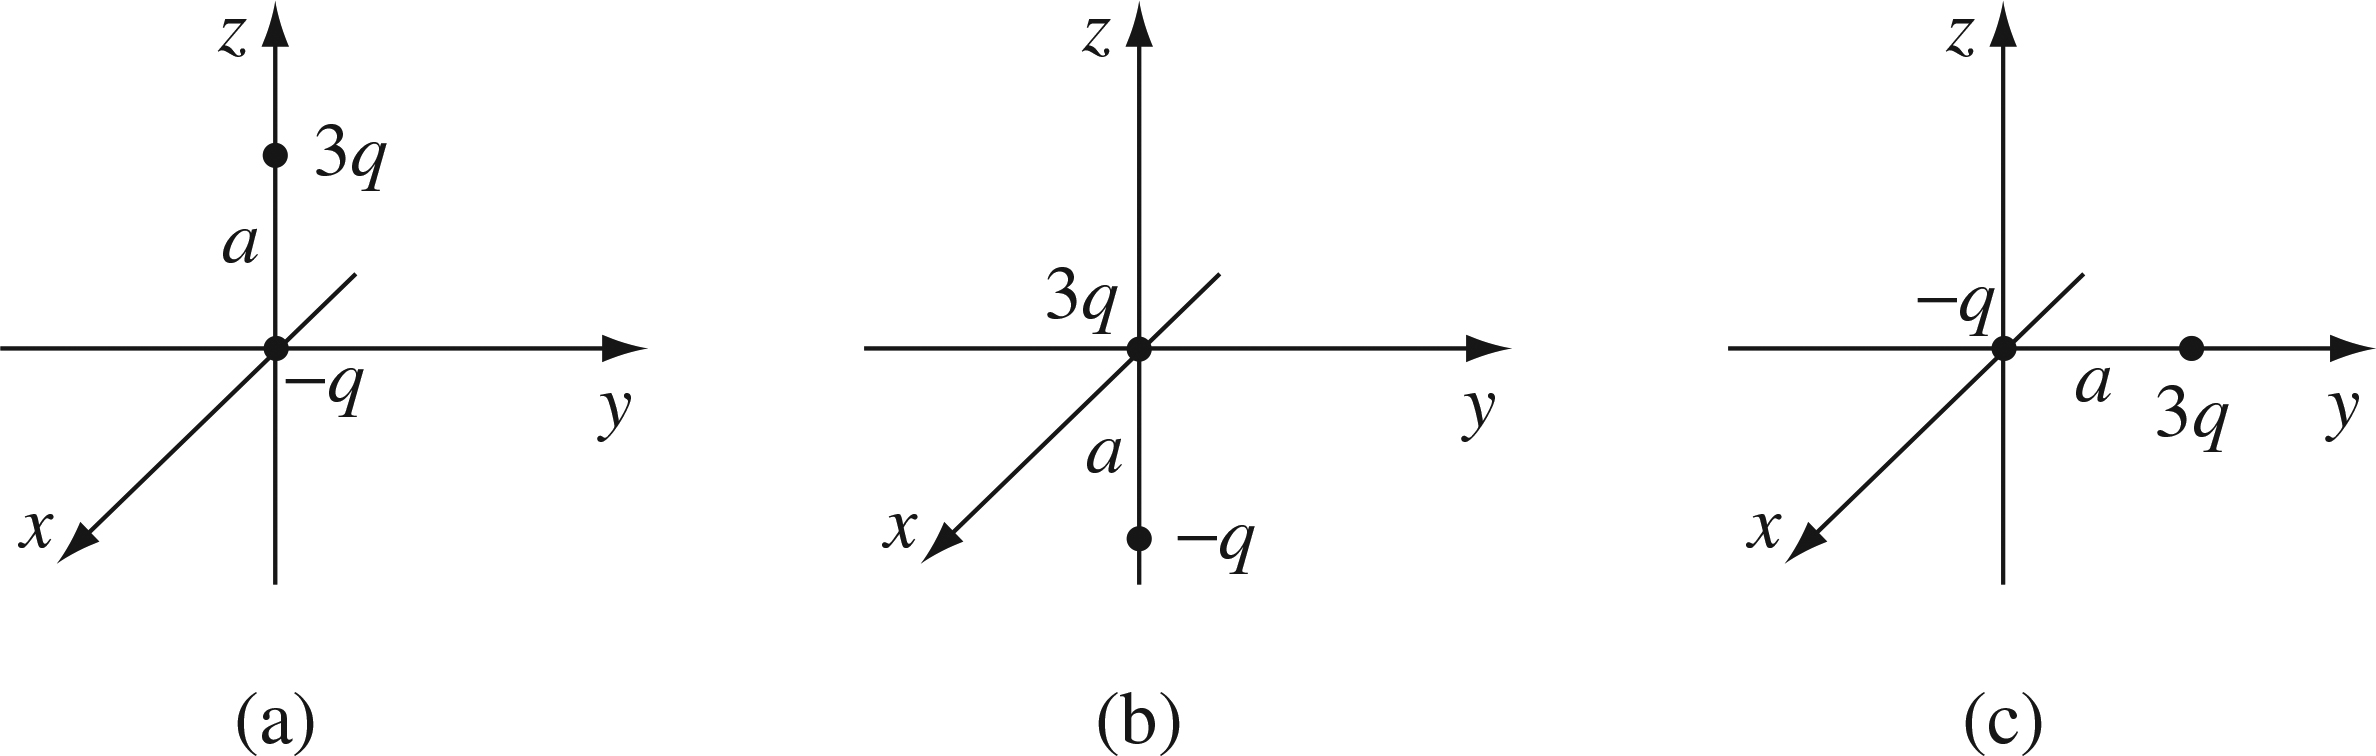
\includegraphics[width=0.65\textwidth]{figures/3_35.jpg}
\caption{\label{fig:dipoles} (Left) An arrangement of four charges near the origin.  (Right, a-c) An arrangement of two charges near the origin, oriented three different ways.}
\end{figure}
\end{enumerate}

\end{document}
